\usepackage{ucll-code}
\usepackage{emerald}
\usepackage[T1]{fontenc}

\title{\cpp: Introduction}
\author{Fr\'ed\'eric Vogels}



\begin{document}

{
  \setbeamercolor{background canvas}{bg=black}
  \ECFJD
  \begin{frame}<handout:0>[plain]
    \begin{center}
      \begin{tikzpicture}[white]
        % \path[use as bounding box] (-5,0) rectangle (5,8);
        \visible<2->{
          \node at (0,8) {
            Please allow me to introduce myself\dots
          };
        }
        \visible<3->{
          \node[anchor=north] (den-bjarne) at (0,7.5) {
            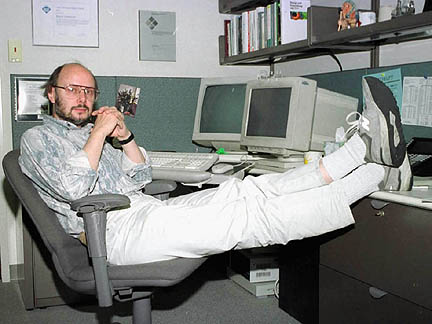
\includegraphics[width=5cm]{BjarneStroustrup.jpg}
          };
        }
        \visible<4->{
          \node[anchor=north] (wealth) at (den-bjarne.south) {
            I'm a man of wealth and taste
          };
        }
        \visible<5->{
          \node[anchor=north] (around) at (wealth.south) {
            I've been around for a long, long year            
          };
        }
        \visible<6->{
          \node[anchor=north] at (around.south) {
            Stole many a man's soul to waste
          };
        }
      \end{tikzpicture}
    \end{center}
  \end{frame}

  \begin{frame}<handout:0>[plain]
    \begin{center}
      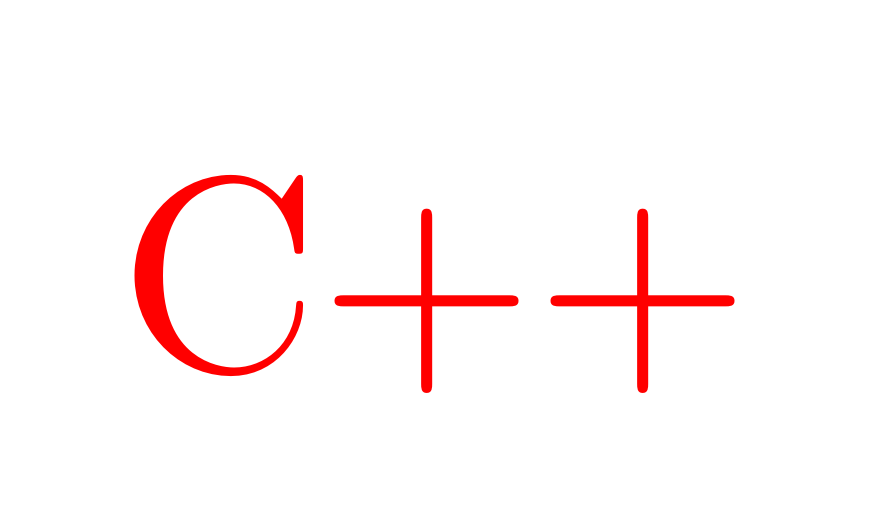
\begin{tikzpicture}[white]
        \node[font=\large] at (0,5) {Bjarne Stroustrup};
        \node at (0,4.5) {presents};
        \node[scale=10,red] at (0,2) {C++};
      \end{tikzpicture}
    \end{center}
  \end{frame}
}

\begin{frame}<beamer:0>
	\titlepage
\end{frame}

\begin{frame}
  \frametitle{The Good}
  \begin{itemize}
    \item It is a very powerful language
    \item Many very advanced language features
    \item Very efficient, because
          \begin{itemize}
            \item You get full control
            \item Compilers are very, very good at optimising
          \end{itemize}
    \item Exists on any platform
    \item Many existing libraries
    \item Used by many (= lots of helpful resources)
          \begin{itemize}
            \item Most games are made in \cpp\ (efficiency)
            \item Most OSs are written in C/\cpp\ (full control)
          \end{itemize}
  \end{itemize}
\end{frame}

\begin{frame}
  \frametitle{The Bad}
  \begin{itemize}
    \item \cpp\ is a \emph{very} difficult language
          \begin{itemize}
            \item Many rules
            \item Complex rules
            \item Inconsistent rules
          \end{itemize}
    \item Those who like \cpp\ generally do not understand it \\
          (or are masochists)
    \item No safety measures
    \item Mistakes are ``punished'' in the sense that they are not!
          \begin{itemize}
            \item The app merrily goes on when mistakes occur
            \item The error only becomes apparent later
          \end{itemize}
    \item Low productivity
          \begin{itemize}
            \item While the code may run fast, it is written slowly
          \end{itemize}
  \end{itemize}
\end{frame}

\begin{frame}
  \frametitle{The Ugly}
  \begin{itemize}
    \item The joys of undefined behaviour
    \item Cryptic compiler errors
    \item \cpp\ = three language for the price of one
          \begin{itemize}
            \item Preprocessor
            \item Templates
            \item ``Regular'' code
          \end{itemize}
    \item IDE support is difficult
  \end{itemize}
\end{frame}


\begin{frame}
  \frametitle{Language Versions and Compilers}
  \begin{columns}
    \begin{column}{5cm}
      \structure{Language versions}
      \begin{itemize}
        \item 1972: C
        \item Cfront: C with classes
        \item 1983: \cpp
        \item 1989: \cpp 2.0
        \item \cpp98
        \item \cpp03
        \item \cpp11
        \item \cpp14
        \item \cpp17
      \end{itemize}
    \end{column}
    \begin{column}{5cm}
      \structure{Compilers}
      \begin{itemize}
        \item MSVC
        \item GCC
        \item Clang
        \item Intel \cpp
        \item HP aCC
        \item Sun/Oracle \cpp
        \item Digital Mars \cpp
        \item Borland (defunct)
        \item Watcom (defunct)
      \end{itemize}
    \end{column}
  \end{columns}
  \begin{center}
    Different compilers support \link{http://en.cppreference.com/w/cpp/compiler_support}{different features}
    of different language versions
  \end{center}
\end{frame}

\begin{frame}
  \frametitle{Unwieldiness}
  \begin{itemize}
    \item Very complex specification
    \item \link{http://www.open-std.org/jtc1/sc22/wg21/docs/papers/2012/n3337.pdf}{Current standard}
          counts 1300+ pages 
    \item Compilers have different interpretations of the standard
    \item Different compilers support different sets of features
    \item Compilers can introduce their own features
    \item Compilers are \emph{very} complex, hence sometimes buggy
  \end{itemize}
\end{frame}

\begin{frame}
  \frametitle{C and \cpp}
  \structure{\cpp's greatest strength is its compatibility with C}
  \begin{itemize}
    \item Familiar syntax
    \item Existing code can be reused
  \end{itemize}
  \vskip5mm
  \structure{\cpp's greatest weakness is its compatibility with C}
  \begin{itemize}
    \item Inherits C's weaknesses
    \item Leads to inconsistencies in language
  \end{itemize}
  \vskip5mm
  \structure{Irony}
  \begin{itemize}
    \item C itself has changed and has introduced incompatibilities
  \end{itemize}
\end{frame}

\begin{frame}
  \frametitle{Java vs \cpp}
  \structure{Java}
  \begin{itemize}
    \item Primary design goal: security
    \item Ease of use
    \item Programmers are fallible mentality
  \end{itemize}
  \vskip5mm
  \structure{\cpp}
  \begin{itemize}
    \item Primary design goal: efficiency
    \item Programmers are gods mentality
  \end{itemize}
\end{frame}

\begin{frame}
  \frametitle{Java vs \cpp: Array Indexing}
  \code[language=c++14,width=5cm]{array-out-of-bounds.cpp}
  \structure{Java}
  \begin{itemize}
    \item No array indexing goes unchecked
    \item \texttt{ArrayIndexOutOfBounds} thrown in your face
  \end{itemize}
  \vskip2mm
  \structure{\cpp}
  \begin{itemize}
    \item No checks whatsoever
    \item Undefined behaviour
    \item Possibly overwrites a random other variable
  \end{itemize}
\end{frame}

\begin{frame}
  \frametitle{Java vs \cpp: Null Pointers}
  \code[language=java,width=5cm]{null.java}
  \structure{Java}
  \begin{itemize}
    \item No member access goes unchecked
    \item \texttt{NullPointereException} thrown in your face
  \end{itemize}
  \vskip2mm
  \structure{\cpp}
  \begin{itemize}
    \item No checks whatsoever
    \item Undefined behaviour
    \item Possibly runs some random code
  \end{itemize}
\end{frame}

\begin{frame}
  \frametitle{Java vs \cpp: Null Pointers}
  \code[language=java,width=5cm]{private.java}
  \structure{Java}
  \begin{itemize}
    \item \texttt{x} is safely locked away
    \item No way to access it (in Java)
  \end{itemize}
  \vskip2mm
  \structure{\cpp}
  \begin{itemize}
    \item Very easy to circumvent
    \item It's more what you'd call a guideline than an actual rule
  \end{itemize}
\end{frame}

\begin{frame}
  \frametitle{Java vs \cpp: Null Pointers}
  \structure{Java}
  \begin{itemize}
    \item Memory safe
    \item Can't peek nor poke around in arbitrary memory
  \end{itemize}
  \vskip2mm
  \structure{\cpp}
  \code[language=c++14]{memory.cpp}
  \begin{itemize}
    \item Whoops!
    \item Overwrites entire memory space
  \end{itemize}
\end{frame}

\begin{frame}
  \frametitle{Java vs \cpp: Garbage Collection}
  \code[language=java]{allocation.java}
  \structure{Java}
  \begin{itemize}
    \item Lost object
    \item Garbage collector will find and recycle it
  \end{itemize}
  \vskip2mm
  \structure{\cpp}
  \begin{itemize}
    \item Lost is lost, no safe way to recuperate it
    \item Memory leak
    \item You need to manually free the object's memory
  \end{itemize}
\end{frame}

\begin{frame}
  \frametitle{Java vs \cpp: Casting}
  \code[language=java]{casting.java}
  \structure{Java}
  \begin{itemize}
    \item Every object knows its (dynamic) type
    \item Casts are checked at runtime
    \item \texttt{ClassCastException} if wrong cast
  \end{itemize}
  \vskip2mm
  \structure{\cpp}
  \begin{itemize}
    \item Many different casts
    \item Some check, some don't
    \item You \emph{can} force a cast to any type you want
  \end{itemize}
\end{frame}

\begin{frame}
  \frametitle{Java vs \cpp: Primitive/Fundamental Types}
  \code[language=java]{primitive-types.java}
  \structure{Java}
  \begin{itemize}
    \item Integers are guaranteed to be two-complement 32 bit
    \item Effect of overflow are predictable
  \end{itemize}
  \vskip2mm
  \structure{\cpp}
  \begin{itemize}
    \item No specific internal representation guaranteed \link{http://www.open-std.org/jtc1/sc22/wg21/docs/papers/2012/n3337.pdf}{\tiny\cpp11 \S 3.9.1/2}
    \item Undefined behaviour
  \end{itemize}
\end{frame}

\begin{frame}
  \frametitle{Java vs \cpp: Type Safety}
  \code[language=java]{primitive-types.java}
  \structure{Java}
  \begin{itemize}
    \item Integers are guaranteed to be two-complement 32 bit
    \item Effects of overflow are predictable
  \end{itemize}
  \vskip2mm
  \structure{\cpp}
  \begin{itemize}
    \item No specific internal representation guaranteed \link{http://www.open-std.org/jtc1/sc22/wg21/docs/papers/2012/n3337.pdf}{\tiny\cpp11 \S 3.9.1/2}
    \item Undefined behaviour
  \end{itemize}
\end{frame}

\begin{frame}
  \frametitle{Morality of this Presentation}
  \begin{itemize}
    \item \cpp\ makes no compromises: efficiency \"uber alles
    \item Throw all your assumptions overboard
    \item Take necessary safety precautions
  \end{itemize}
\end{frame}

\begin{frame}
  \frametitle{Why \cpp?}
  \begin{center}
    \begin{tabular}{cc}
      \textbf{Ranking} & \textbf{Taal} \\
      \toprule
      1 & Java \\
      2 & C \\
      3 & C++ \\
      4 & C$^\sharp$ \\
      5 & Python \\
    \end{tabular}
    \vskip5mm
    \link{http://www.tiobe.com/tiobe-index/}{\tiny TIOBE Index for January 2017}
  \end{center}
\end{frame}

\begin{frame}
  \frametitle{Applications Written in \cpp}
  \begin{columns}
    \column{5cm}
    \begin{itemize}
      \item Browsers
            \begin{itemize}
              \item Chrome
              \item Internet Explorer
              \item Firefox
              \item Safari
              \item Opera
            \end{itemize}
      \item MS Office
            \begin{itemize}
              \item Word
              \item Excel
              \item Access
              \item Powerpoint
              \item Outlook
            \end{itemize}
    \end{itemize}
    \column{5cm}
    \begin{itemize}
      \item Windows/Linux GUIs
      \item JVM
      \item MySQL
      \item MS SQL Server
      \item MongoDB
      \item Photoshop
      \item Games
            \begin{itemize}
              \item Id Tech 5, 6
              \item Unreal Engine
              \item Most games
            \end{itemize}
    \end{itemize}
  \end{columns}
  \vskip4mm
  \structure{In summary}
  \begin{center}
    Most desktop applications
  \end{center}
\end{frame}

\begin{frame}
  \frametitle{Why \cpp}
  \begin{itemize}
    \item Java takes many choices away from you
    \item \cpp\ gives you more options
    \item \cpp\ allows you to better understand the why behind things
  \end{itemize}
\end{frame}

\begin{frame}
  \frametitle{Example}
  \code[language=java]{arguments.java}
  \begin{itemize}
    \item Java always passes arguments by value
    \item Functions receive a \emph{copy}
    \item Impossible to write a \texttt{swap} function
  \end{itemize}
  \code[language=java]{swap.java}
\end{frame}

\begin{frame}
  \frametitle{Example}
  \code[language=c++14]{swap.cpp}
  \begin{itemize}
    \item \cpp\ allows you to choose
    \item You can pass by value, by pointer or by reference
    \item You can give readonly access
  \end{itemize}
\end{frame}

\begin{frame}
  \frametitle{Other Examples}
  \structure{Inheritance}
  \begin{itemize}
    \item Java only supports single inheritance
    \item \cpp\ offers multiple inheritance
    \item \cpp\ offers public, protected, private inheritance
  \end{itemize}
  \vskip5mm
  \structure{Overriding}
  \begin{itemize}
    \item In Java all methods are overridable
    \item \cpp\ there are ``regular'' and virtual methods
  \end{itemize}
\end{frame}

\begin{frame}
  \frametitle{Other Examples}
  \structure{Generics}
  \begin{itemize}
    \item Java only class types
    \item \cpp\ allows any type to be used
    \item \cpp\ supports specialisation
    \item \cpp\ supports template metaprogramming
  \end{itemize}
  \vskip5mm
  \structure{Allocation}
  \begin{itemize}
    \item Three types of allocation
    \item Java picks which type is used for what
    \item \cpp\ allows you to choose yourself
  \end{itemize}
\end{frame}

\end{document}


%%% Local Variables:
%%% mode: latex
%%% TeX-master: "cpp-intro"
%%% End:
